\myparagraph{Purpose}
The main feature of \textit{AutomatedSOS} is to check the health status of the user and to detect any critical situation.
\textit{AutomatedSOS} monitors the health status of the subscribed customers and, when such parameters are below certain thresholds, sends to the location of the customer an ambulance, guaranteeing a reaction time of less than 5 seconds from the time the parameters are below the threshold.

\myparagraph{Scenario 1}
For a couple of days Vittorio felt very tired and affected of sickness. While he was walking in his house his heartbeat went down and he lied down on the floor. Luckily he had installed \textit{AutomatedSOS} application.
The application detected a critical situation, it managed to track Vittorio position and it called the ambulace.
The ambulace arrived very quickly and luckily the paramedics with a cardiac massage saved Vittorio that was carried to the hospital.

\myparagraph{Scenario 2}
Cristiano is a professional runner. He decides to install on his phone \textit{AutomatedSOS} to keep trace of his health status and avoid any possible critical situation when he runs.
One day, while he was running, \textit{AutomatedSOS} went in an alerted status but after only 1 second the application came back in a normal status and stayed in the normal status for all the duration of the run.
Probably it was an abnormal device measure of life value, so \textit{AutomatedSOS} did not call the ambulance.

\myparagraph{Use Case}
The \textit{Critical Situation} use case is analyzed in Table \ref{table:criticalSituationTable}.

\myparagraph{Activity Diagram}
The \textit{Critical Situation} activity diagram is shown in Figure \ref{img:criticalSituationActivityDiagram}.

\myparagraph{Mockup}
The \textit{Critical Situation} mockup is shown in Figure \ref{img:criticalSituationMockup}.

\myparagraph{Functional requirements}
\begin{enumerate}
  \item The system must guarantee a reaction time of less than 5 seconds from the time it detects an alerted situation;
  \item The system must send the location of the customer to an ambulance;
  \item The system must be in an alerted status when maximum pressure value of the customer is more than 170 mmHg and minimum pressure value is more than 100 mmHg;
  \item The system must be in an alerted status when the heartbeat is lower than 45 bmp or it is higher than 120 bpm;
  \item If the system goes in an alerted status it has to increase the life parameters detection frequency.
\end{enumerate}

\begin{center}
\begin{table}[H]
\begin{tabular}{ | l | p{0.75\linewidth} | }
  \hline
    Actor & \textbf{User} \\ \hline
    Goal & \textbf{[G.8]} \\ \hline
    Input Condition & The system goes in an alerted status \\ \hline
    Event Flow & \begin{minipage}[t]{0.7\textwidth}
      \begin{enumerate}
        \item The system gets the GPS position of the \textbf{User};
        \item The system increases parameters detection with a frequence of 3 detection per second;
        \item The system shows an alert message on the \textbf{User}'s device (smartwatch or similar).
      \end{enumerate}
    \smallskip
  \end{minipage} \\ \hline
  Output Condition & The system calls an ambulance and it sends the location to the called ambulance if it is in an alert status from 3 seconds. \\ \hline
  Exceptions & \begin{minipage}[t]{0.7\textwidth}
    \begin{itemize}
      \smallskip
      \item If functional requirement 2 is not satisfied the system notifies the ambulance about the detected position error and sends the last detected position;
      \item If the system could not detect life parameters of the \textbf{User}, it invites him/her to check the status and the conncetion of his/her device with a warning message.
    \end{itemize}
    \smallskip
  \end{minipage}  \\ \hline
\end{tabular}
\caption{\textit{Critical Situation} use case}
\label{table:criticalSituationTable}
\end{table}
\end{center}

\begin{figure}[H]
\begin{center}
  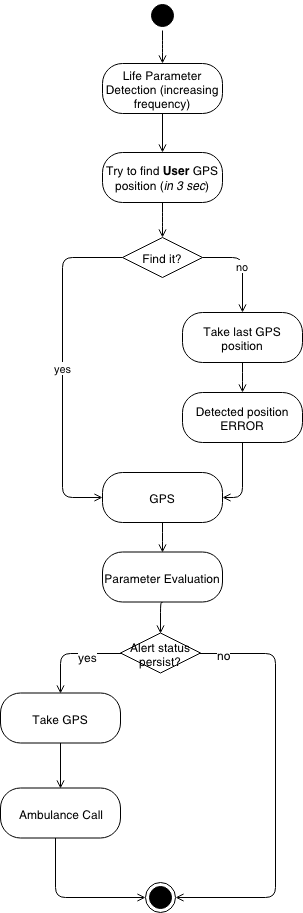
\includegraphics[height=0.6\paperheight]{img/activity/Alert.png}
  \hspace{0.05\linewidth}
  \centering
  \caption{\textit{Critical Situation} activity diagram from system's point of view}
  \label{img:criticalSituationActivityDiagram}
\end{center}
\end{figure}

\begin{figure}[H]
\begin{center}
  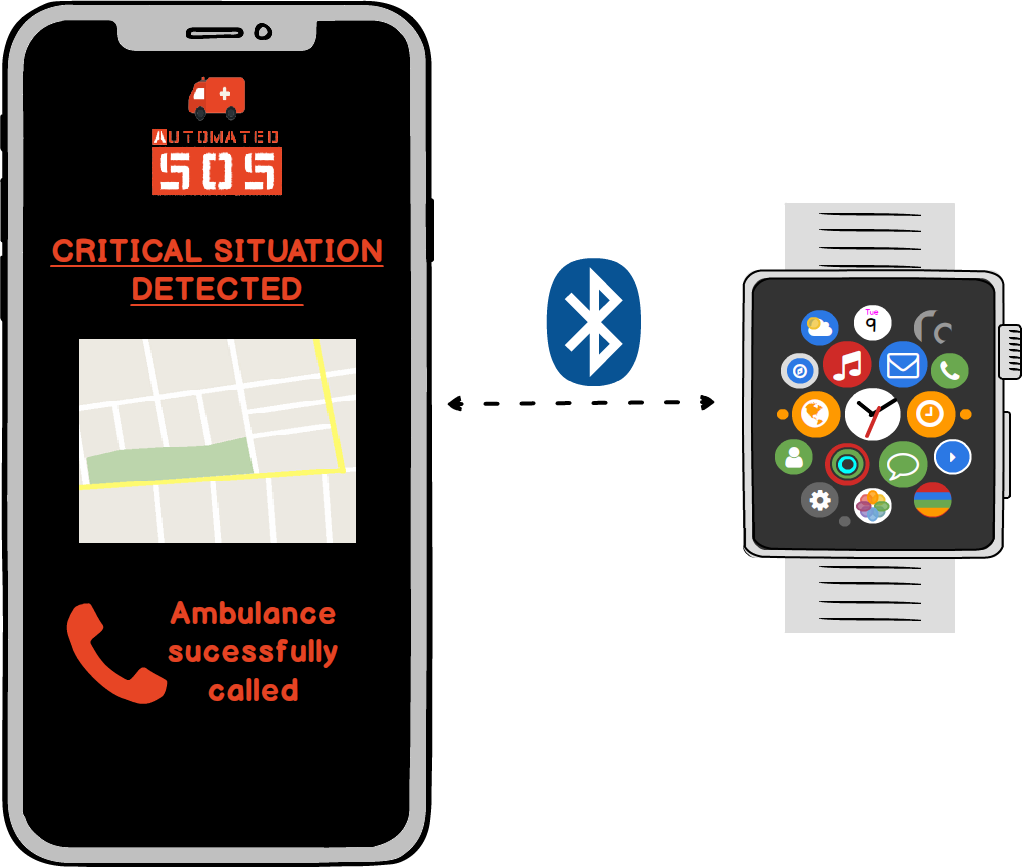
\includegraphics[width=\textwidth]{img/mockup/Critical_Situation.png}
  \hspace{0.05\linewidth}
  \centering
  \caption{\textit{Critical Situation} mockup}
  \label{img:criticalSituationMockup}
\end{center}
\end{figure}
